\section{Evaluation of Implementation Characteristics}
\label{sec:exp}

%\begin{itemize}
%	\item CPU results
%		\begin{itemize}
%			\item Insert-only workload
%			\item Pop-only workload
%			\item Mix workload
%		\end{itemize}
%	\item Xeon Phi results
%		\begin{itemize}
%			\item Insert-only workload
%			\item Pop-only workload
%			\item Mix workload
%		\end{itemize}
%	\item Explanation on why we are not fast
%\end{itemize}

%we should change this subsection title
\subsection{Memory allocation micro-benchmark}
We performed a microbenchmark to evaluate the memory allocation process in the XeonPhi. We did three different types of mememory allocation: First, we used the primites offered by the programming language, then we used compiler hints offered by the Intel Thread Building Blocks to use its scalable allocator implementation, and finally we allocated the memory needed sequentially using compiler hints too. These options are described below.

\mypar{C++ memory allocation primitives}
These are optimized for sequential case. They were designed with two main objectives: use efficiently memory space and minimize CPU overhead. However, these objectives do not target achieving good parallel performance. Modern hardware provides larger memory sizes, but also a bigger gap between CPU and memory speed. Thus, cache locality and avoidance of false sharing play a more important role.

\mypar{Intel TBB scalable allocator}
It uses \textit{thread-private heaps} to reduce the amount of code that needs synchronization and also false sharing. Each thread allocates its own copy of heap structures and accesses it via thread-specific data (TSD) using corresponding system APIs.
The allocator gets 1MB chunks from the operating system and divides them into 16K-byte aligned blocks. Then, it places these blocks initially in a global heap of free blocks. Memory requested is not returned to the operating system (but only in large allocation cases). Thus, it can make sure that memory is reused. Additional blocks are requested if a thread does not find free objects in the blocks of its own heap and there are no available blocks in the global heap~\cite{_thefoundations,Hudson:2006:MST:1133956.1133967}.
To use the scalable allocator offered by Intel TBB we had to link two libraries:
\begin{description}
	\item[-ltbb] To use the Intel TBB library.
	\item[-ltbbmalloc] To use the scalable allocator offered by the Intel TBB library.
\end{description}
 
\mypar{Sequential allocation with compiler hints}
Every node in our skip list contains an array of pointers to the next nodes depending on the level each node belongs to. This means that parts of this array might fall into different cache lines. Thus, our data structure can suffer more from cache misses and false sharing. We designed each skip list node to contain an empty array and allocating only the pointers that it will actually need (listing~\ref{lst:freenode}). In addition to that, the usage of Intel TBB allocator helps us ensuring that these nodes will be cache-aligned (listing~\ref{lst:fn_alloc}).

\begin{lstlisting}[language=C++,basicstyle=\tt\footnotesize,captionpos=b,caption=Lock free node structure,label=lst:freenode,morekeywords={*, size_t}]
template <typename T>  struct LockFreeNode
{	
	T data;
	int	level;
	AtomicRef<LockFreeNode>	next[0];
};
\end{lstlisting}

\begin{lstlisting}[language=C++,basicstyle=\tt\footnotesize,captionpos=b,caption=Memory allocation instruction for array of atomic references,label=lst:fn_alloc, morekeywords={*, size_t}]

scalable_malloc(
sizeof(LockFreeNode) 
+ 
((arrayLength + 1) * sizeof(AtomicRef<LockFreeNode>))
)
\end{lstlisting}

\mypar{Memory allocation microbenchmnark}
We designed our microbenchmark to allocate ten million skip list nodes and measure the time it takes to complete the task on the XeonPhi. When using the regular memory allocation method, we experienced really high latency but when we used Intel TBB scalable allocator we obtained a 24, and 38 times improvemente for using TBB library, and a sequential allocation with Intel TBB allocator respectively. The results are displayed on figure~\ref{fig:mem_alloc}.


% explain data + graph 
\begin{figure}
	\centering
  	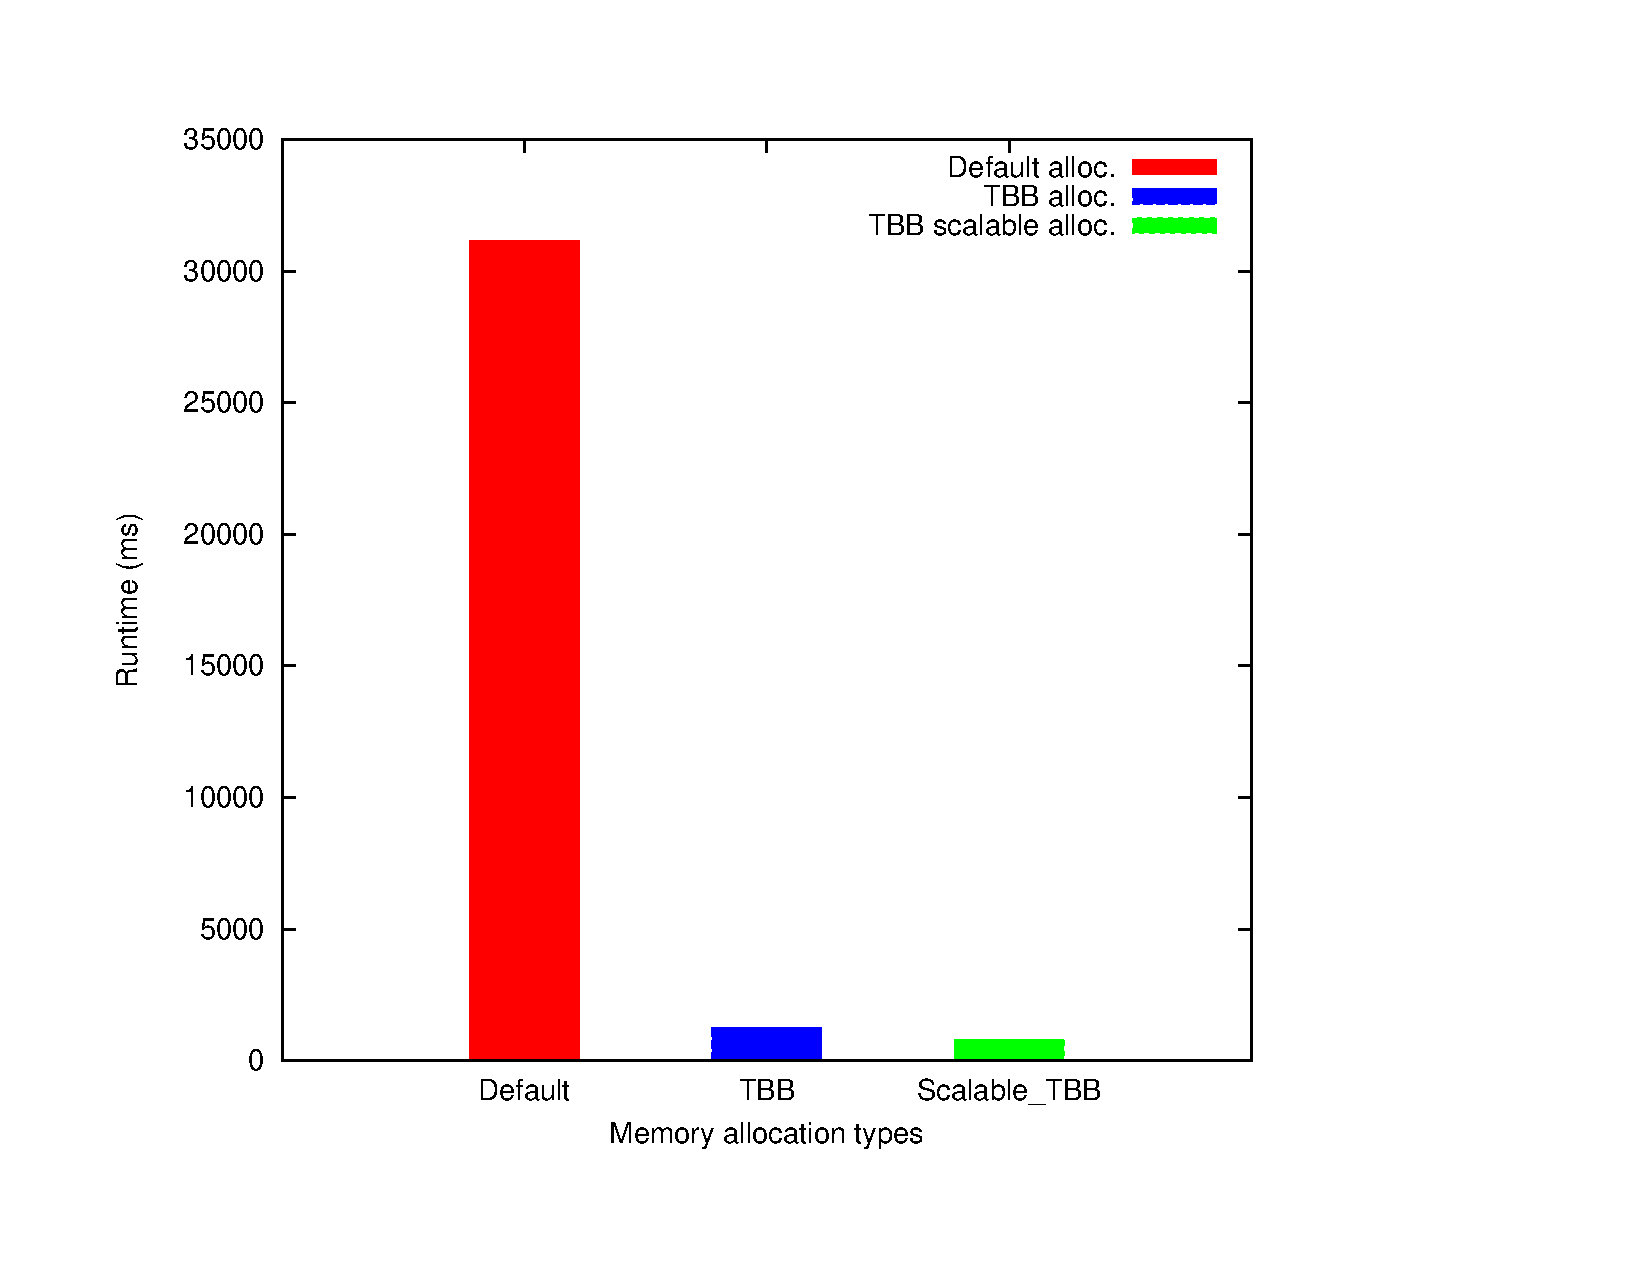
\includegraphics[scale=0.35]{../plots/mem_alloc/mem_alloc.pdf}
	\caption{Memory allocation runtime among a regular allocation, using compiler hints, and using sequential allocation with compiler hints}
	\label{fig:mem_alloc}
\end{figure}


\mypar{Operational intensity}
% recap of operational intensity
Operational intensity is defined as the ratio of the number of instructions executed to the number of memory accesses(look for citation?). If there exist many instructions per memory access, then the program is considered to have a high computational intensity i.e. compute bounded. On the other hand, if there are a small number of instructions are executed per memory access, then the program is considered to have a low computational intensity i.e. memory bounded.

% why we think it matters in our case
Our project goal was to design a simple, yet effective, priority queue. Thus, we expected to have an operational intensity dominated mainly by the number of memory accesses, and aimed to improve this. Having to move data around has a different impact on CPU architectures. We will describe and explain how our data structure behaves on Intel Haswell microarchitecture (Intel Core i7-4558U) and on Sandy BridgeE microarchitecture (Intel Core i7-3820K). 

% Differences between these two microarchitectures
%TODO fix bib
The Intel Haswell microarchiteture is the successor of Ivy Bridge which in turn is the successor of Sandy Bridge. They have several differences but they also share many commonalities. One of the biggest change is the memory hierarchy implemented on the Intel Haswell. The cache bandwidth doubled and its memory sytem can now perform two loads and one store per cycle. The Haswell's L1 load bandwidth is of 64 bytes/cycle, its L1 store bandwidth is of 32 bytes/cycle and also L2 bandwidth to L1 has doubled (from 32 bytes/cycle to 64 bytes/cycle). Other relevant improvements are the ones related to the Translation Look-aside Buffer (TLB) which in Haswell has access to 2M shared pages. The page entry also doubled in Haswell as well as the associativity; It went from a 4-way associative TLB in 
 Bridge to a 8-way associative TLB in Haswell. These changes are summarized on table~\ref{tab:haswell_ivy}.
%~\cite{http://ijcsit.com/docs/Volume%204/vol4Issue3/ijcsit2013040321.pdf, http://www.agner.org/optimize/microarchitecture.pdf, http://web.eecs.utk.edu/courses/fall2013/cosc530/CS530Project_intel.pdf}

\begin{table}[ht]
\footnotesize
\begin{tabular}{|l|l|l|ll}
\cline{1-3}
\multicolumn{1}{|c|}{\textbf{Metric}} & \multicolumn{1}{c|}{\textbf{Sandy BridgeE}} & \multicolumn{1}{c|}{\textbf{Haswell}} &  &  \\ \cline{1-3}
L1 Load Bandwidth                     & 32 Bytes/cycle                           & 64 Bytes/cycle                        &  &  \\ \cline{1-3}
L1 Store bandwidth                    & 16 Bytes/cycle                           & 32 Bytes/cycle                        &  &  \\ \cline{1-3}
L2 Bandwidth to L1                    & 32 Bytes/cycle                           & 64 Bytes/cycle                        &  &  \\ \cline{1-3}
L2 Unified TLB                        & 4K:512, 4-way                            & 4k+2M shared: 1024, 8-way             &  &  \\ \cline{1-3}
\end{tabular}
\caption{Cache operation differences between Intel Haswell and Intel SandyBridgeE}
\label{tab:haswell_ivy}
\end{table}

% describe cache structure
In addition to core cache size, latency, and bandwith improvements, the Intel Haswell microarchitecture has also improved its ICache prefetch algorithms, and the way it handles conflicts. It uses hardware transactions i.e. it uses hardware to keep track of which cache lines have been read from and which have been written to. L1 cache tracks addresses read/written from/to respectively in the transactional region and it may evict address but without loss of tracking. Data conflicts occur if at least one request is doing a write, but it is detected at cache line granularity and using existing cache coherence protocol.

%~\cite{http://pages.cs.wisc.edu/~rajwar/papers/rajwar_qconsf2012.pdf}
%~\cite{http://www.realworldtech.com/haswell-cpu/5/
%the Ivy Bridge has 1333MHz DRAM while the Haswell has 2133MHz DRAM
While running our priority queue benchmark on these two different architectures, we observed different behaviours. The running times when using an Intel IvyBridge processor dramatically increases due the increase of the total amount of instructions and cache misses. Everytime we need to perform an insertion, we first have to search for the adecuate place within the SkipList. The average of the SkipList nodes fit in a 64-byte cache line but the ones containing pointers in upper levels don't. On the other hand, when we used an Intel Haswell processor, running times were much less than in the Sandy BridgeE processor. This is mainly due to the improvements done on cache operations. In this case, our data structure can take advantage of such improvements by loading more SkipList nodes into the caches that can also be used by other threads.

% explain data + graph + core architecture
\begin{figure}
	\centering
  	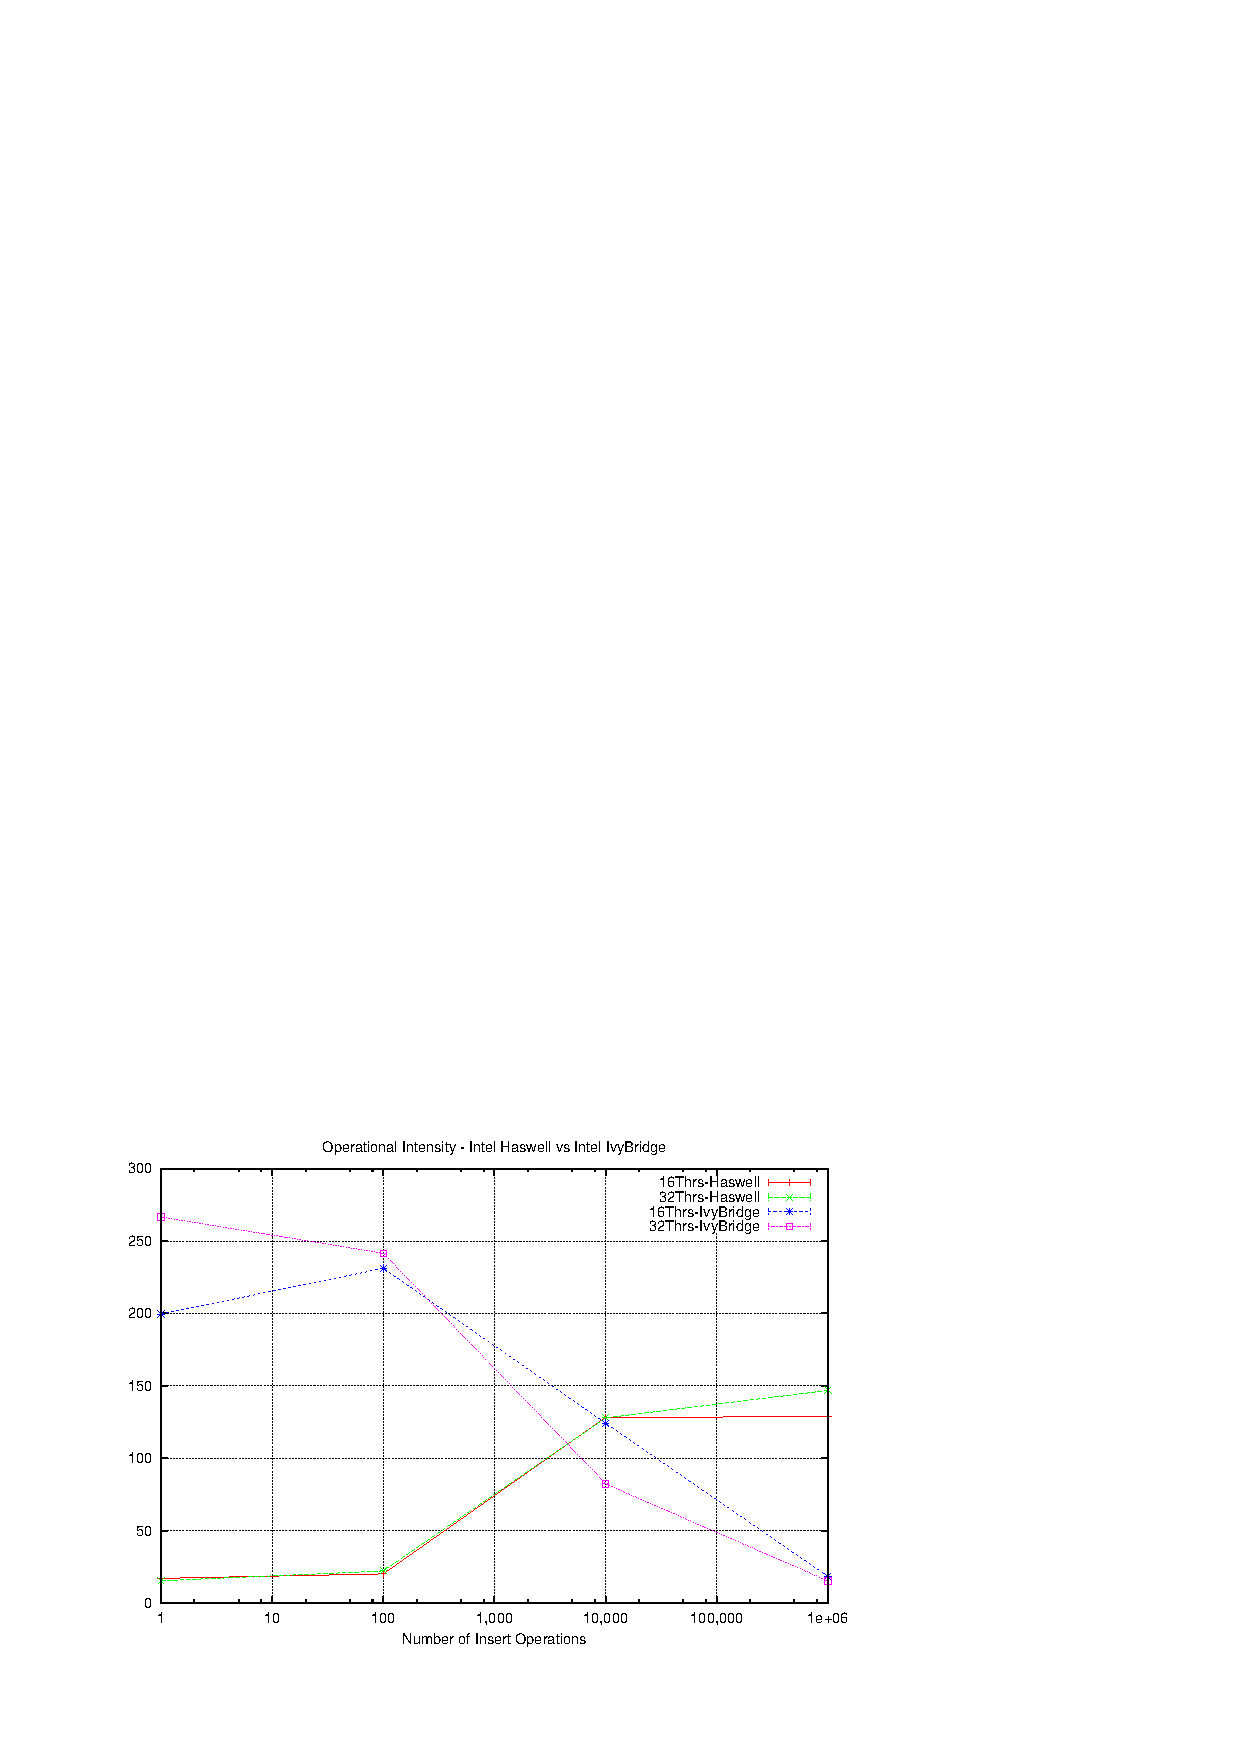
\includegraphics[scale=0.3]{../plots/haswell-ivybridge/haswell_ivybridge.pdf}
	\caption{Op. Intensity in Intel Haswell and Intel Sandy BridgeE microarchitectures}
	\label{fig:haswell_ivybridge}
\end{figure}

Figure~\ref{fig:haswell_ivybridge} shows how operational intensity behaves when running different amounts of insert operations over such microarchitectures. It can be noted that when performing a small number of operations, our data structure is CPU bounded on an Sandy BridgeE processor, but memory bounded on a Haswell processor. This is because in the former we have a small number of cache-misses against a really high number of instructions whether in the latter we observed a low operational intensity because we need less number of instructions for performing such tasks. When we increase the number of operations, the Sandy BridgeE processor gets many more cache-misses compared to the Haswell one. Thus, in the former one our data structure becomes memory bounded and in the latter one CPU bounded.

\section{Experiments on Workloads}
COMPILER on Einstein sucks\\
The experiments were conducted on two different systems. First a CPU-based system equipped with an Intel Xeon E3-1245 running 4 Coreas at 3.4\,Ghz, second a MIC, the Intel Xeon Phi 7XXX. To allow comparison the experiment parameters used were the same on both platforms. For each experiment five iterations were averaged and their standard deviation was computed.\\
Three types of workload were executed, \textit{mixed}, \textit{push} and \textit{pop}. For the mixed and pop the priority queue was prepopulated with 1000$\times$threads in the former and 10\,Mio. elements in the latter. Prepopulation was not included in the measured runtime. The \textit{mixed} workload chooses for each operation with probability of 50\% either a push or pop operation. The number of threads is varied from 1 to 240 in steps of 20 while the number of operations per threads stays constant.


\subsection{Evaluation on Core i7}
\begin{figure*}[t]
	\centering
	\begin{subfigure}[b]{0.3\textwidth}
		\centering
		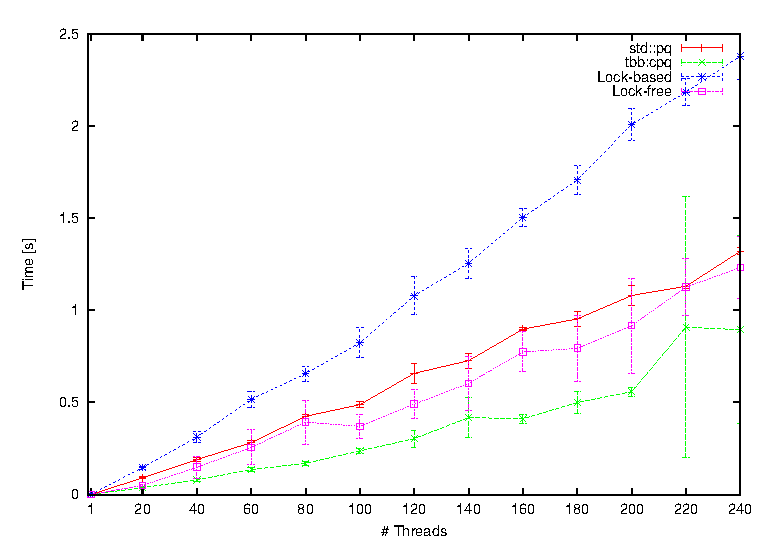
\includegraphics[width=\textwidth]{../plots/i7_mixed/runtime_mixed_i7}
		\caption{Mixed Workload}
		\label{fig:i7_mixed}
	\end{subfigure}
	\hfill
	\begin{subfigure}[b]{0.3\textwidth}
		\centering
		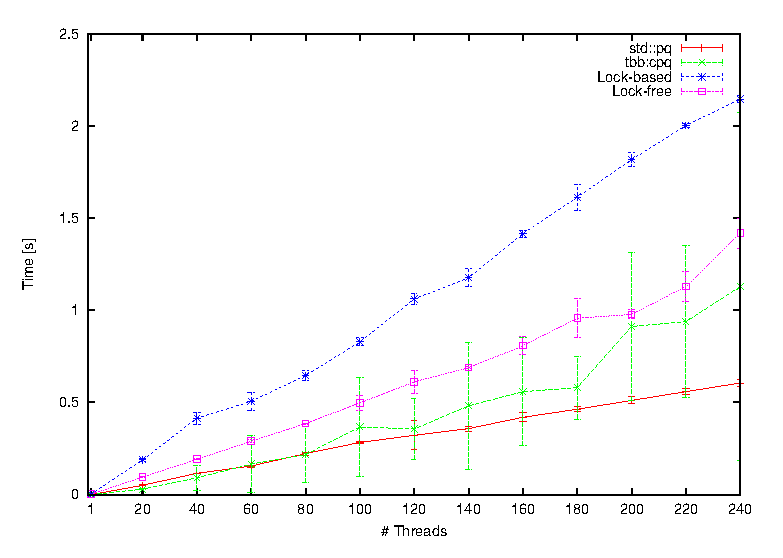
\includegraphics[width=\textwidth]{../plots/i7_push/runtime_push_i7}
		\caption{PUSH}
		\label{fig:i7_push}
	\end{subfigure}
	\hfill
	\begin{subfigure}[b]{0.3\textwidth}
		\centering
		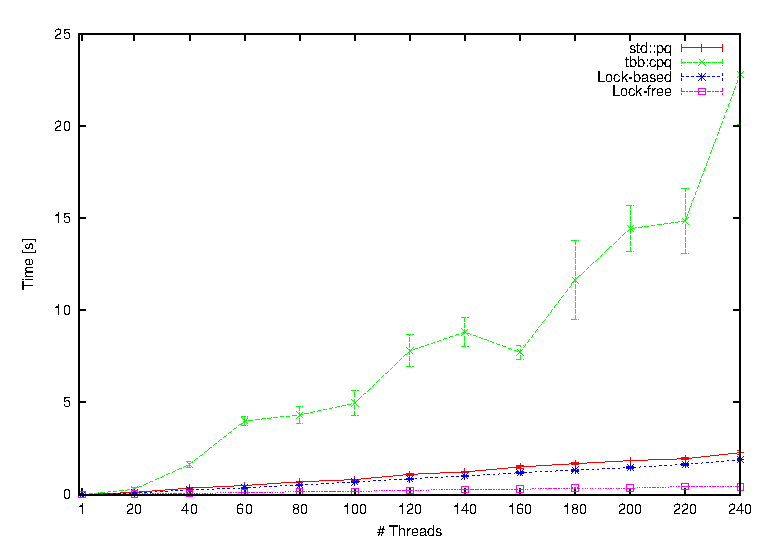
\includegraphics[width=\textwidth]{../plots/i7_pop/runtime_pop_i7}
		\caption{POP}
		\label{fig:i7_pop}
	\end{subfigure}
	\caption{Evaluation on Intel Core E3-1245}
	\label{fig:eval_i7}
\end{figure*}
\figurename~\ref{fig:eval_i7} shows the run-times for executing the three workloads on a Xeon Haswell system. All variants are performing and behaving similar in the mixed and push workload except for the lock-based implementation which struggles more to scale with the number of threads. Our lock-free implementation is very close to the baseline implementations and shows similar behavior when adding more threads. In the pop workload all four data structures behave very similar, this time the our lock-free implementation with a pop operation in O(1) and lazy-deletion shows the best runtime by a small margin.


\subsection{Evaluation on Xeon Phi}
\begin{figure*}[t]
	\centering
	\begin{subfigure}[b]{0.3\textwidth}
		\centering
		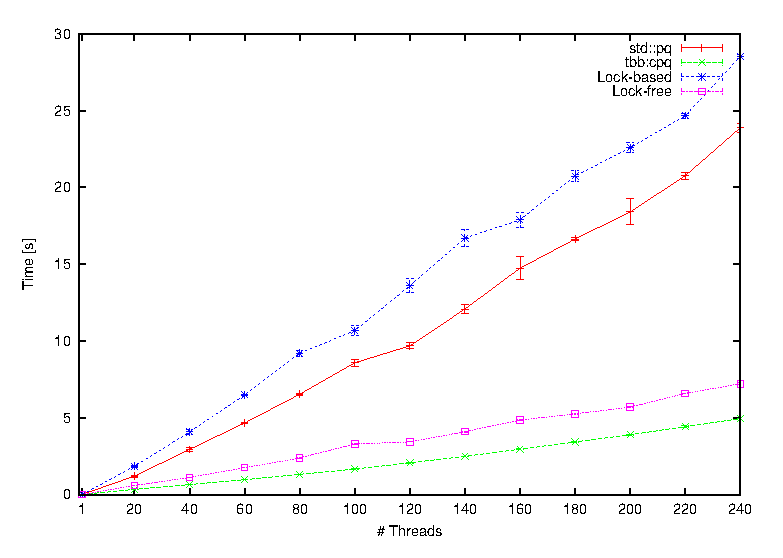
\includegraphics[width=\textwidth]{../plots/xp_mixed/runtime_mixed}
		\caption{Mixed Workload}
		\label{fig:xp_mixed}
	\end{subfigure}
	\hfill
	\begin{subfigure}[b]{0.3\textwidth}
		\centering
		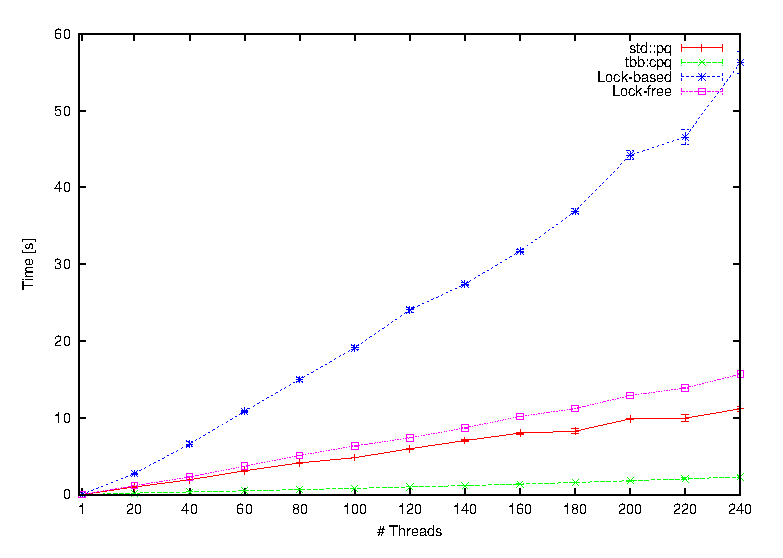
\includegraphics[width=\textwidth]{../plots/xp_push/runtime_push}
		\caption{PUSH}
		\label{fig:xp_push}
	\end{subfigure}
	\hfill
	\begin{subfigure}[b]{0.3\textwidth}
		\centering
		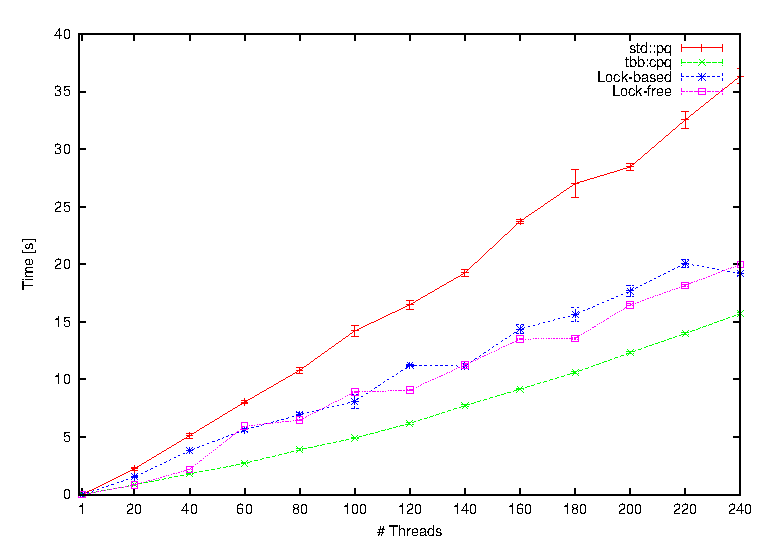
\includegraphics[width=\textwidth]{../plots/xp_pop/runtime_pop}
		\caption{POP}
		\label{fig:xp_pop}
	\end{subfigure}
	\caption{Evaluation on Xeon Phi}
	\label{fig:eval_xp}
\end{figure*}
The same three worklaods were also run on the Xeon Phi, the measured run-times are plotted in \figurename~\ref{fig:eval_xp}. In the mixed workload the tbb and the lock-free priority queue behave similarly well. The other two implementations behave worse. From the push rsp. pop workload we see that the longer runtime in the lock-based implementation originates from bad performance for the push operation while for the std::priority\_queue the pop operation is the case for the long runtime. The tbb::concurrent\_queue behaves well in all three workloads, our lock-free implementation shows almost the same behavior with a slightly increased runtime.\\

Comparing the two platforms against each other we can see that in general the same work is about one magnitude quicker on the CPU.


\subsection{Comparison}
\begin{figure}[t]
	\centering
	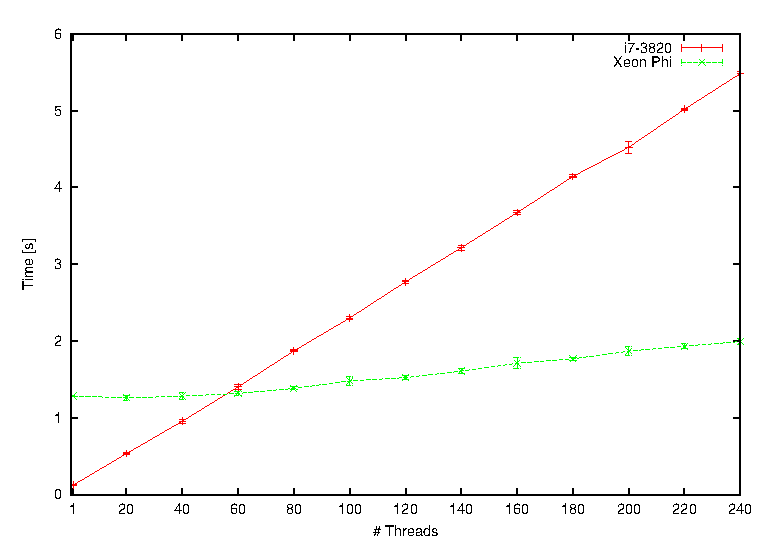
\includegraphics[width=0.9\columnwidth]{../plots/comp_contains/runtime_contains}
	\caption{Comparison memory bandwidth}
	\label{fig:comp_contains}
\end{figure}
The previous experiments show that the same workload performs on a x86 CPU roughly a magnitutde better than on the Xeon Phi architecture. There are multiple reasons for these, ...\\ %cache coherence, memory allocation is more expensive, ....
The Xeon Phi does not only offer computational power but also has a very high memory bandwidth, similar to GPUs, based on GDDR5 which should outperform typical DDR3 main memory. To compare memory bandwidth, we implented a contains function which is querying for elements and checks if they exist. The sturcture of the priority queue is unchanged during this operation, such that dirty cache-lines are omitted. \figurename~\ref{fig:comp_contains} show the lock-free priority queue running on an Intel Core i7-3820 and the Xeon Phi. For all runs the queue was prepopulated with 10\,Mio. elements, each threads executed 100'000 \textit{contains} operations. As can be seen in the graph the runtime on the Xeon Phi only increases slightly with the number of threads, in contrast on the Intel Core i7-3820 it increases roughly linearly. This means that on the x86 architecture the \textit{contains} operation is memory bound already with a single thread. The Xeon Phi seems to guarantee a fixed bandwidth for each of its hardware cores, such that we can scale the number of threads up without being limited by the memory bandwidth.\\


\subsection{Operational intensity in different microarchitectures}
% recap of operational intensity
Operational intensity is defined as the ratio of the number of instructions executed to the number of memory accesses(look for citation?). If there exist many instructions per memory access, then the program is considered to have a high computational intensity i.e. compute bounded. On the other hand, if there are a small number of instructions are executed per memory access, then the program is considered to have a low computational intensity i.e. memory bounded.

% why we think it matters in our case
Our project goal was to design a simple, yet effective, priority queue. Thus, we expected to have an operational intensity dominated mainly by the number of memory accesses, and aimed to improve this. Having to move data around has a different impact on CPU architectures. We will describe and explain how our data structure behaves on Intel Haswell microarchitecture (Intel Core i7-4558U) and on Sandy BridgeE microarchitecture (Intel Core i7-3820K). 

% Differences between these two microarchitectures
%TODO fix bib
The Intel Haswell microarchiteture is the successor of Ivy Bridge which in turn is the successor of Sandy Bridge. They have several differences but they also share many commonalities. One of the biggest change is the memory hierarchy implemented on the Intel Haswell. The cache bandwidth doubled and its memory sytem can now perform two loads and one store per cycle. The Haswell's L1 load bandwidth is of 64 bytes/cycle, its L1 store bandwidth is of 32 bytes/cycle and also L2 bandwidth to L1 has doubled (from 32 bytes/cycle to 64 bytes/cycle). Other relevant improvements are the ones related to the Translation Look-aside Buffer (TLB) which in Haswell has access to 2M shared pages. The page entry also doubled in Haswell as well as the associativity; It went from a 4-way associative TLB in 
 Bridge to a 8-way associative TLB in Haswell. These changes are summarized on table~\ref{tab:haswell_ivy}.
%~\cite{http://ijcsit.com/docs/Volume%204/vol4Issue3/ijcsit2013040321.pdf, http://www.agner.org/optimize/microarchitecture.pdf, http://web.eecs.utk.edu/courses/fall2013/cosc530/CS530Project_intel.pdf}

\begin{table}[ht]
\footnotesize
\begin{tabular}{|l|l|l|ll}
\cline{1-3}
\multicolumn{1}{|c|}{\textbf{Metric}} & \multicolumn{1}{c|}{\textbf{Sandy BridgeE}} & \multicolumn{1}{c|}{\textbf{Haswell}} &  &  \\ \cline{1-3}
L1 Load Bandwidth                     & 32 Bytes/cycle                           & 64 Bytes/cycle                        &  &  \\ \cline{1-3}
L1 Store bandwidth                    & 16 Bytes/cycle                           & 32 Bytes/cycle                        &  &  \\ \cline{1-3}
L2 Bandwidth to L1                    & 32 Bytes/cycle                           & 64 Bytes/cycle                        &  &  \\ \cline{1-3}
L2 Unified TLB                        & 4K:512, 4-way                            & 4k+2M shared: 1024, 8-way             &  &  \\ \cline{1-3}
\end{tabular}
\caption{Cache operation differences between Intel Haswell and Intel SandyBridgeE}
\label{tab:haswell_ivy}
\end{table}

% describe cache structure
In addition to core cache size, latency, and bandwith improvements, the Intel Haswell microarchitecture has also improved its ICache prefetch algorithms, and the way it handles conflicts. It uses hardware transactions i.e. it uses hardware to keep track of which cache lines have been read from and which have been written to. L1 cache tracks addresses read/written from/to respectively in the transactional region and it may evict address but without loss of tracking. Data conflicts occur if at least one request is doing a write, but it is detected at cache line granularity and using existing cache coherence protocol.

%~\cite{http://pages.cs.wisc.edu/~rajwar/papers/rajwar_qconsf2012.pdf}
%~\cite{http://www.realworldtech.com/haswell-cpu/5/
%the Ivy Bridge has 1333MHz DRAM while the Haswell has 2133MHz DRAM
While running our priority queue benchmark on these two different architectures, we observed different behaviours. The running times when using an Intel IvyBridge processor dramatically increases due the increase of the total amount of instructions and cache misses. Everytime we need to perform an insertion, we first have to search for the adecuate place within the SkipList. The average of the SkipList nodes fit in a 64-byte cache line but the ones containing pointers in upper levels don't. On the other hand, when we used an Intel Haswell processor, running times were much less than in the Sandy BridgeE processor. This is mainly due to the improvements done on cache operations. In this case, our data structure can take advantage of such improvements by loading more SkipList nodes into the caches that can also be used by other threads.

% explain data + graph + core architecture
\begin{figure}\centering
%  	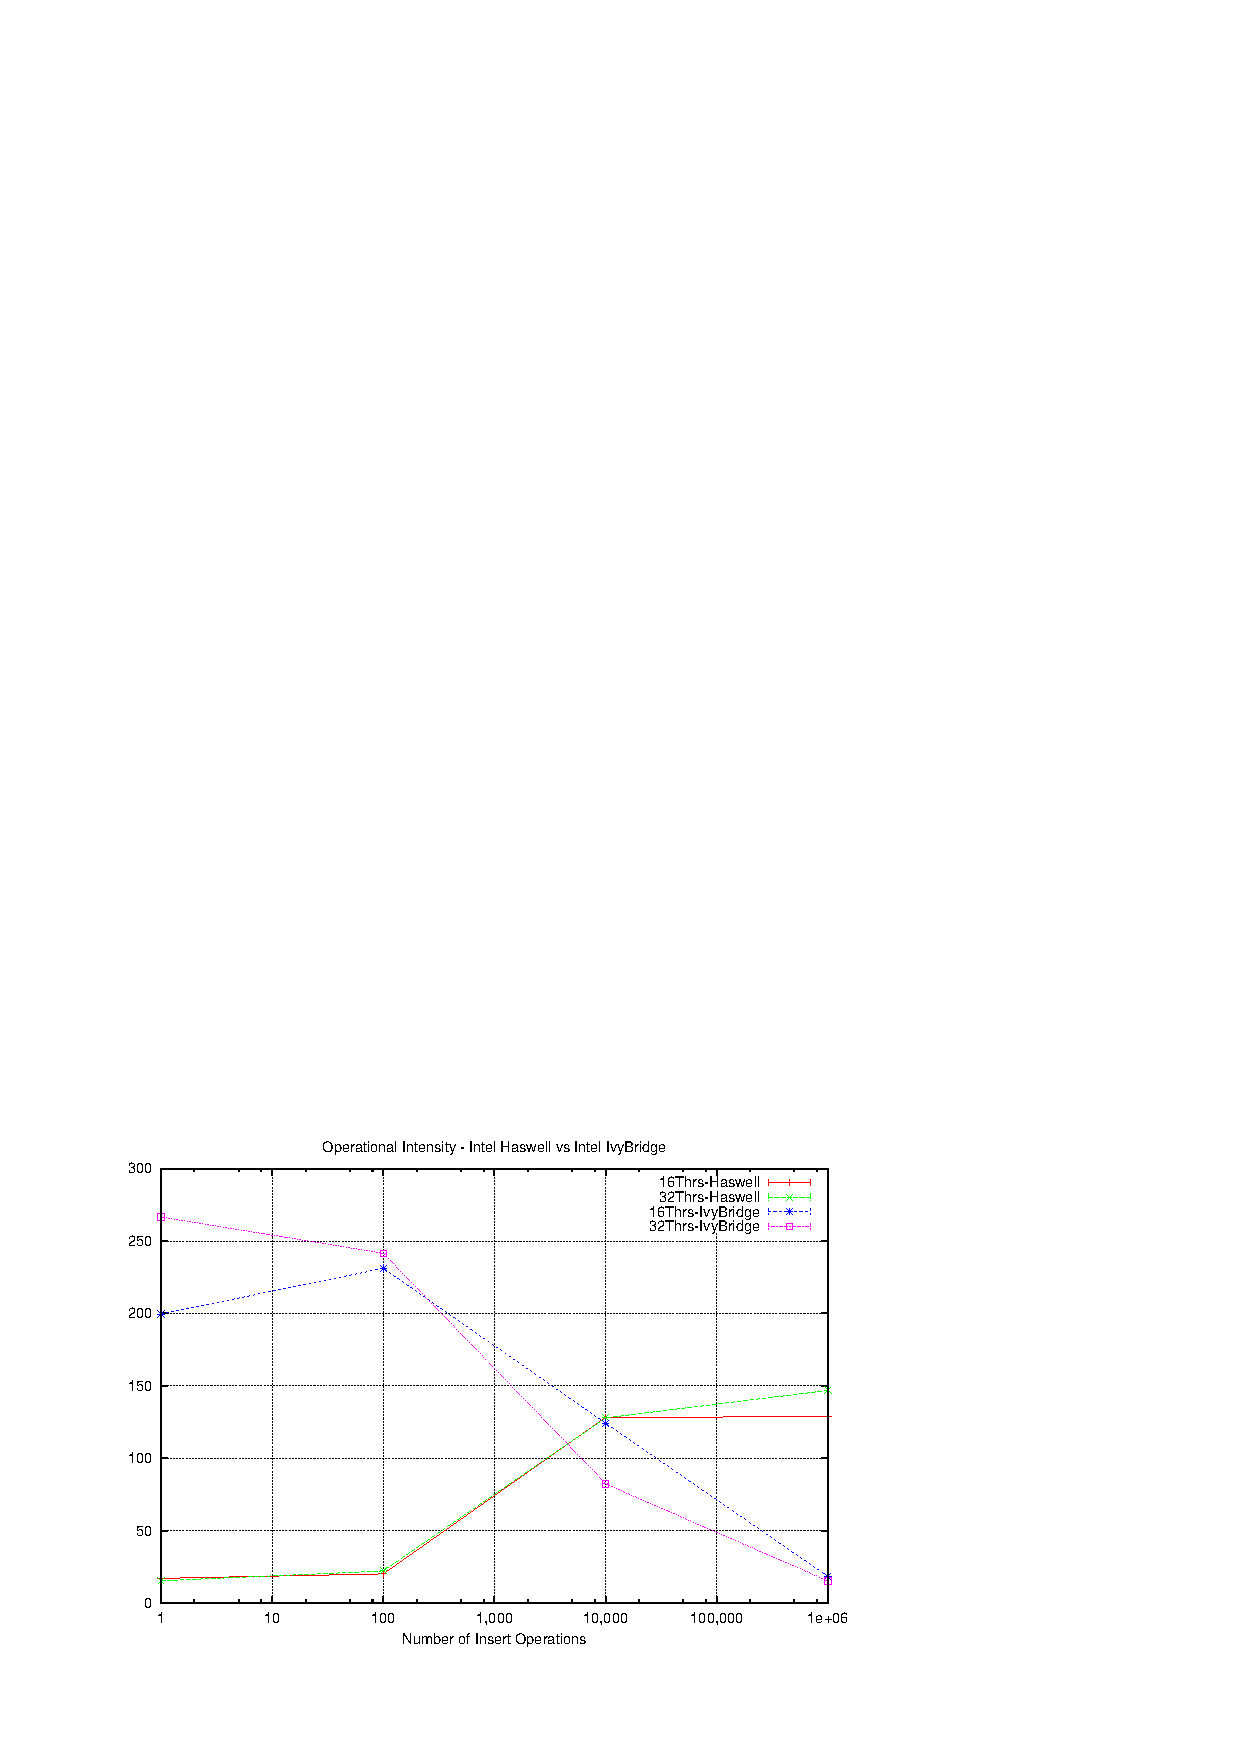
\includegraphics[scale=0.3]{../plots/haswell-ivybridge/haswell_ivybridge.pdf}
	\caption{Op. Intensity in Intel Haswell and Intel Sandy BridgeE microarchitectures}
	\label{fig:haswell_ivybridge}
\end{figure}

Figure~\ref{fig:haswell_ivybridge} shows how operational intensity behaves when running different amounts of insert operations over such microarchitectures. It can be noted that when performing a small number of operations, our data structure is CPU bounded on an Sandy BridgeE processor, but memory bounded on a Haswell processor. This is because in the former we have a small number of cache-misses against a really high number of instructions whether in the latter we observed a low operational intensity because we need less number of instructions for performing such tasks. When we increase the number of operations, the Sandy BridgeE processor gets many more cache-misses compared to the Haswell one. Thus, in the former one our data structure becomes memory bounded and in the latter one CPU bounded.
